\documentclass[11pt]{article} % 
\usepackage[pdftex]{graphicx}
\usepackage{fullpage}
\usepackage{graphicx}
\usepackage{graphics}
\usepackage{psfrag}
\usepackage{pgf}
\usepackage{color}
\usepackage{tikz}
\usetikzlibrary{arrows,automata}
\usepackage[latin1]{inputenc}
\usepackage{amsthm}
\usepackage{amsmath,amssymb}
\usepackage{enumerate}
\setlength{\textwidth}{6.5in}
\setlength{\textheight}{9in}
\newcommand{\N}{\mathbb{N}}
\newcommand{\Z}{\mathbb{Z}}
\newcommand{\R}{\mathbb{R}}
\newcommand{\Q}{\mathbb{Q}}
\newcommand{\C}{\mathbb{C}}
\newcommand{\PP}{\mathbb{P}}
\newcommand{\tab}{\;\;\;\;\;}
\newcommand{\inv}{^{-1}}
\newcommand{\tr}{\textrm}
\newcommand{\lc}{\sqcup}
\newcommand{\var}{\tr{Var}}
\newcommand{\cov}{\tr{Cov}}

\begin{document}

\hfill Robert Johns

\hfill February 6, 2014

\begin{center} {\Large CSCI 678: Statistical Analysis of Simulation Models}\\{\large Homework 3}\end{center}

\begin{enumerate}

%1
\item Modify the M/G/1 queueing simulation program from Assignment 1 to print out the sample autocorrelations for the wait times for lags 1 to 20 using the formulas given on page 2.29.  Make 3 replications using different sets of random variables and plot three correlograms on one set of axes.

{\bf Solution:} See attached code \texttt{ams3a.c}

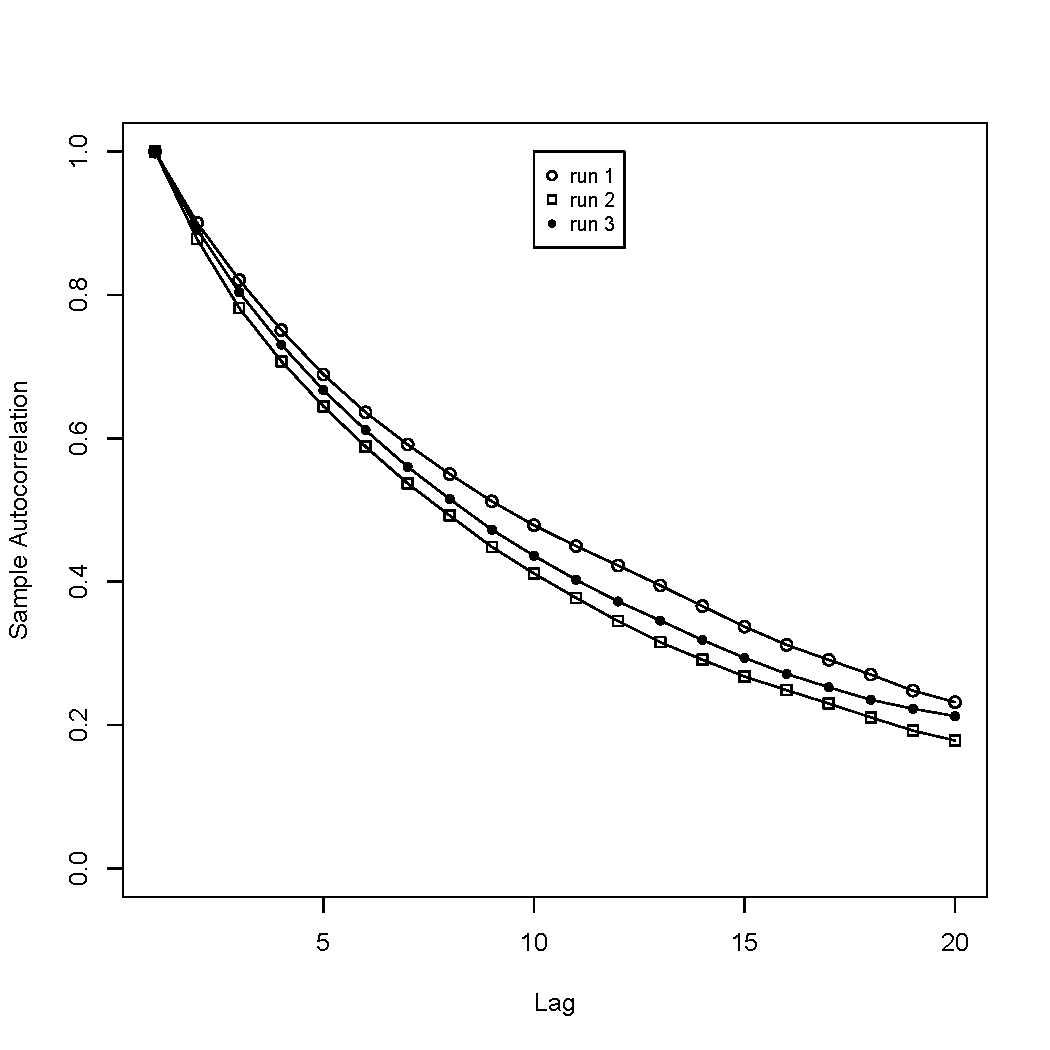
\includegraphics[scale = .6]{plot.pdf}

%%%%%
%2
\item For the exponential distribution: $f(x) = \frac{1}{\alpha}e^{-x/\alpha},\;\; x \ge 0$

\begin{enumerate}

%2a
\item Find the mgf.

{\bf Solution:} $M_X(t) = E[e^{tx}] = \int_0^\infty\frac{1}{\alpha}e^{x(t - 1/\alpha)}\;dx = (1 - \alpha t)\inv$

%2b
\item Generate the first four raw moments. using the result from part (a)

{\bf Solution:} From the formula $E[X^r] = \left.\frac{d^rm_X(t)}{dx^r}\right|_{t=0}$, we get

$E(X) = m_X'(0) = \left.\frac{\beta}{(\beta*t-1)^2}\right|_{t=0} = \beta$

$E(X^2) = m_X''(0) = \left.\frac{-2\beta}{(\beta*t-1)^3}\right|_{t=0} = -2\beta$

$E(X^3) = m_X'''(0) = \left.\frac{6\beta^3}{(\beta*t-1)^4}\right|_{t=0} = 6\beta^3$

$E(X^4) = m_X^{(4)}(0) = \left.\frac{24\beta^4}{(\beta*t-1)^5}\right|_{t=0} = 24\beta^4$

%2c
\item What is the mode of the exponential distribution?

{\bf Solution:} It will be the maximum value of the pdf of the exponential distribution. Examining the distribution graphically, we see that this happens at $x = 0$.

%2d
\item What is the median of the exponential distribution?

{\bf Solution:} First, we need the cdf.  To do this, we evaluate $\int_0^mf(w)\;dw = 1 - e^{-m/\beta}$.  Then we set the equation equal to 1/2 and solve.  We get $1/2 = 1 - e^{-m/\beta}$, or $e^{-m/\beta} = 1/2$, or $-m/\beta = \ln(1/2)$, or $m = -\beta\ln(1/2)$.

%2e
\item Give an expression for determining a fractile of an exponential R.V.

{\bf Solution:} We see, following our process from part (d), that the only effect that the specific fractile had on our answer was the term inside the natural logarithm.  An appropriate expression for the $p$th fractile, therefore, would be $x_p = -\beta\ln(p)$.

\end{enumerate}

%%%%%
%3
\item State the following complex numbers in each of the three standard forms:

\begin{enumerate}

%3a
\item $3 + 4i$

{\bf Solution:} $a + bi: 3 + 4i$

Polar: $5e^{.6435i}$

Sines, Cosines: $5(\cos(.6435) + i\sin(.6435))$

%3b
\item $10e^{(\pi i)/4}$

{\bf Solution:} $a + bi: 5\sqrt{2} + 5\sqrt{2}i$

Polar: $10e^{(\pi i)/4}$

Sines, Cosines: $10(\cos(\pi/4) + i\sin(\pi/4))$

%3c
\item $4(\cos(2\pi/3) + i\sin(2\pi/3))$

{\bf Solution:} $a + bi: -2 + 2\sqrt{3}i$

Polar: $4e^{(2\pi i)/3}$

Sines, Cosines: $4(\cos(2\pi/3) + i\sin(2\pi/3))$

\end{enumerate}

%%%%%
%4
\item Consider independent random variables $Y_1, Y_2$ and $Y_3$.  Using only expectations, variances and covariances, derive (and simplify) expressions for:

\begin{enumerate}

%4a
\item $\cov(Y_1 + Y_3, Y_2 + Y_3)$

{\bf Solution:} We have the shortcut formula for covariance: $\cov(X,Y) = E(XY) - E(X)E(Y)$, which gives us 
$$\cov(Y_1 + Y_3, Y_2 + Y_3) = E[(Y_1 + Y_3)(Y_2 + Y_3)] - E(Y_1 + Y_3)E(Y_2 + Y_3)$$
$$= E(Y_1Y_2 + Y_1Y_3 + Y_2Y_3 + Y_3^2) - [E(Y_1) + E(Y_3)][E(Y_2) + E(Y_3)]$$
$$= E(Y_1Y_2) + E(Y_1Y_3) + E(Y_2Y_3) + E(Y_3^2) - [E(Y_1)E(Y_2) + E(Y_1)E(Y_3) + E(Y_2)E(Y_3) + E(Y_3)^2]$$
$$=[E(Y_1Y_2) - E(Y_1)E(Y_2)] + [E(Y_1Y_3) - E(Y_1)E(Y_3)] + [E(Y_2Y_3) - E(Y_2)E(Y_3)] + [E(Y_3^2) - E(Y_3)^2]$$
$$=\cov(Y_1,Y_2) + \cov(Y_1,Y_3) + \cov(Y_2,Y_3) + \var(Y_3)$$
$$= \var(Y_3)$$

%4b
\item $\rho$ for $(Y_1 + Y_3, Y_2 + Y_3)$

{\bf Solution:} The formula for $\rho$ of two random variables $X$ and $Y$ is $\frac{\cov(X,Y)}{\sigma_X\sigma_Y}$.  So we have
$$\rho = \var(Y_3)/(\sqrt{\var(Y_1 + Y_3)\var(Y_2 +Y_3)})$$
$$= \var(Y_3)/\sqrt{[\var(Y_1) + \var(Y_3)][\var(Y_2) + \var(Y_3)]}$$
$$=\var(Y_3)/\sqrt{\var(Y_1)\var(Y_2) + \var(Y_1)\var(Y_3) + \var(Y_2)\var(Y_3) + \var(Y_3)^2}$$

\end{enumerate}

%%%%%
%5
\item Find the characteristic function for the $U(0,1)$ distribution.  Show that $\phi_x(0) = 1$.

{\bf Solution:} We have $\phi_X(t) = E[e^{itx}] = \int_0^1e^{itx}\;dx$.  Performing a u-substitution, where $u = itx$ and $du = it\;dx$, we have $\int_0^1e^{itx}\;dx = \frac{-i}{t}\int_0^1e^u\;du = \left.\frac{-i}{t}e^{itx}\right|_0^1 = \frac{-i}{t}(e^{it} - 1) = \frac{i}{t}(1 - e^{it}) = \frac{i}{t}(1 - \cos(it) - i\sin(it)) = \frac{i - i\cos(it) + \sin(it)}{t} = \phi_X(t)$

We see that $\phi_X(0) = E[e^{i*0*x}] = E[e^0] = E[1] = 1$

%%%%%
%6
\item Suppose that $X$ and $Y$ are jointly discrete random variables with
$$f(x, y) = \left\{\begin{array}{ll} \frac{2}{n(n+1)} & x = 1, 2, \ldots n; y = 1, 2 \ldots, x \\
0 & \tr{otherwise}\end{array}\right.$$
Find $f_X(x), f_Y(y)$ and determine whether $X$ and $Y$ are independent.

{\bf Solution:} Firstly, a neat party trick tells us that $X$ and $Y$ cannot be independent, because they are not defined on a product space; the space they are defined on is the discrete representation of a triangle.  Now, for the marginals.  A cursory example of the geometry gives us the functions:

$$f_X(x) = \left\{\begin{array}{ll}
\frac{2x}{n(n+1)} & x \in \{1, 2, \ldots, n\}\\
0 & \tr{otherwise}\end{array}\right.$$

$$f_Y(y) = \left\{\begin{array}{ll}
\frac{2(n-y + 1)}{n(n+1)} & y \in \{1, 2, \ldots, n\}\\
0 & \tr{otherwise}\end{array}\right.$$ 

%%%%%%
%7
\item For a single run of the M/G/1 queue simulation from question 1, determine the sample minimum, maximum and the quartiles of the customer wait times by writing the wait times to a file and reading those vales into R.  Submit code in C and R, and the values for the minimum, maximum and quartiles.

{\bf Solution:} See attached code \texttt{asm3b.c}.  The short program \texttt{asm3c.r} is written below.  The results are also printed blow.

$\begin{array}{l   |  l}
Results & Program \\\hline
\texttt{"min:" 1.000149} & \texttt{data <- scan("data.txt")}\\

\texttt{"max:" 24.56443}&\texttt{print("min:")}\\

\texttt{"quartiles"     25\%      50\%      75\% }& \texttt{print(min(data))}\\
\texttt{1.831689 3.040863 5.097327}&\texttt{print("max:")}\\

 & \texttt{print(max(data))}\\

&\texttt{print("quartiles")}\\

&\texttt{print(quantile(data, c(.25, .5, .75	)))}\end{array}$

\end{enumerate}

\end{document}